\chapter{Infrastruktura}

\section{Úvod}
S výjimkou databázového systému je aplikace rozdělena do dvou oddělených vrstev: frontend a backend. Rozhodnutí nevyužít fullstack framework, jako je například Nuxt, je poměrně jednoduché. Tyto dvě vrstvy mohou fungovat zcela odděleně, což umožňuje využití různých verzí technologií a zajišťuje větší flexibilitu při správě a nasazování jednotlivých částí systému.

Toto rozdělení přináší také zásadní výhody z hlediska budoucí rozšiřitelnosti. Aplikace se dá snadno přizpůsobit pro různé platformy – například ji lze rozšířit o mobilní nebo desktopovou aplikaci, aniž by to narušilo stávající strukturu. Díky této modularitě je architektura systému robustnější a lépe připravená na budoucí požadavky. Navzdory rozdělení je projekt uložený v jednom git repozitáři.

\section{Databáze}

% \subsection{Specifikace zadání}

\subsection{Vize}
Navrhovaný systém pro posilovnu bude zajišťovat správu rezervací, uživatelů a vybavení posilovny. Hlavním účelem systému je rezervační konfigurátor, jehož primární funkcí je alokace dostupných přístrojů. Systém integruje algoritmus pro dynamické doporučení optimálních časových intervalů na základě vytíženosti zařízení a přizpůsobený výběr přístrojů na bázi typu tréninku.

\subsection{Role}
Rolí systém podporuje několik. Uživatele rozdělujeme do tří skupin.

\begin{description}
    \item[Zákazník] je role s nejnižšími právy. Zákazník bude representovat osobu, která si v systému bude chtít vytvořit rezervaci
    \item[Trenér] je role která má rozšítěný přístup k systému, je to obyčejný uživatel, který může být přiřazen k rezervaci. Asociaci s rezervací může ale sám zrušit. V zadání tuto roli nemáme popsanou, tudíž se pro tento typ účtu nebude v rámci této bakalářské práce implementovat logika navíc. Prozatím bude fungovat jako obyčejný uživatel, kterého lze přidat k rezervaci jako trenéra.
    \item[Zaměstnanec] je role, která má přístup k administraci, je to role s nejvyššími právy a je schopna přidávat, manipulovat a mazat veškerá data. Bude také mít přístup ke všem statistikám a výpisům.
\end{description}
Tyto skupiny nám zajistí integritu přístupu dat a jejich manipulaci. Pro tento systém není potřeba více rolí, jelikož Zaměstnanců, kteří jsou pověřeni manipulací dat a přístupu do administrace je malé množství, tudíž téměř neomezený přístup k datům má nízké chybové dopady.

\subsection{Popis}
Systém bude primárně zaměřen na chod posilovny, což zahrnuje správu rezervací přístrojů na konkrétní časy a potenciálně i sledování výdělků. Pro zajištění těchto specifikací je potřeba se ujistit, že systém tyto specifikace pokrývá. Systém je postaven na třech pilířích.

\begin{description}
    \item[Uživatelské účty] Většina záznamů v systému vyžaduje uchovávání informací o uživateli. Samotná autentizace a související procesy, jako je ověřování uživatelů, budou řešeny mimo rámec databáze pomocí externích služeb. Nicméně je stále potřeba ukládat dodatečné informace o uživatelích přímo v databázi. Pro tento účel systém obsahuje jednoduchou tabulku s názvem account, která slouží k uchování základních informací o uživatelských účtech, jako jsou identifikátory nebo další nezbytné údaje.
    \item[Rezervace a plán] Jak napovídá samotný název, tabulka rezervace reprezentuje uživatelovu rezervaci, která je vždy vázána na konkrétní den. Každá rezervace je spojená s uživatelem a určitým plánem a může mít přiřazeného trenéra. Plán představuje komplexnější strukturu několika tabulek, které uchovávají podrobné informace o rezervaci, například konkrétní přístroje, časové rozvrhy a další detaily. Plán je tvořen následujícími tabulkami: plan, plan\_category a plan\_machine.
    \item[Přístroje a kategorie] Tabulka machine reprezentuje skutečné posilovací přístroje dostupné v posilovně. Každý přístroj má definované základní informace, jako jsou jeho název a popis, a je spojen s určitým plánem. Vztah mezi přístroji a plánem je typu N:M (mnoho na mnoho), což umožňuje asociaci jednoho přístroje s více plány a naopak. Tento vztah je dále rozšířen o dodatečné informace, jako je počet opakování (repetic), počet sérií (setů) a časové intervaly, zahrnující počáteční a koncový čas cvičení. Dále jsou s každým plánem a přístrojem asociovány kategorie, které jsou uchovávány v tabulce plan\_category. Tyto kategorie umožňují lépe strukturovat a organizovat přístroje a plány podle typu cvičení nebo jiných kritérií, což usnadňuje správu systému, zvyšuje jeho přehlednost a poskytne možnost doporučit Přístroje podle předem vybraných.
\end{description}


\subsection{Datová analýza}

\begin{figure}[h!]
	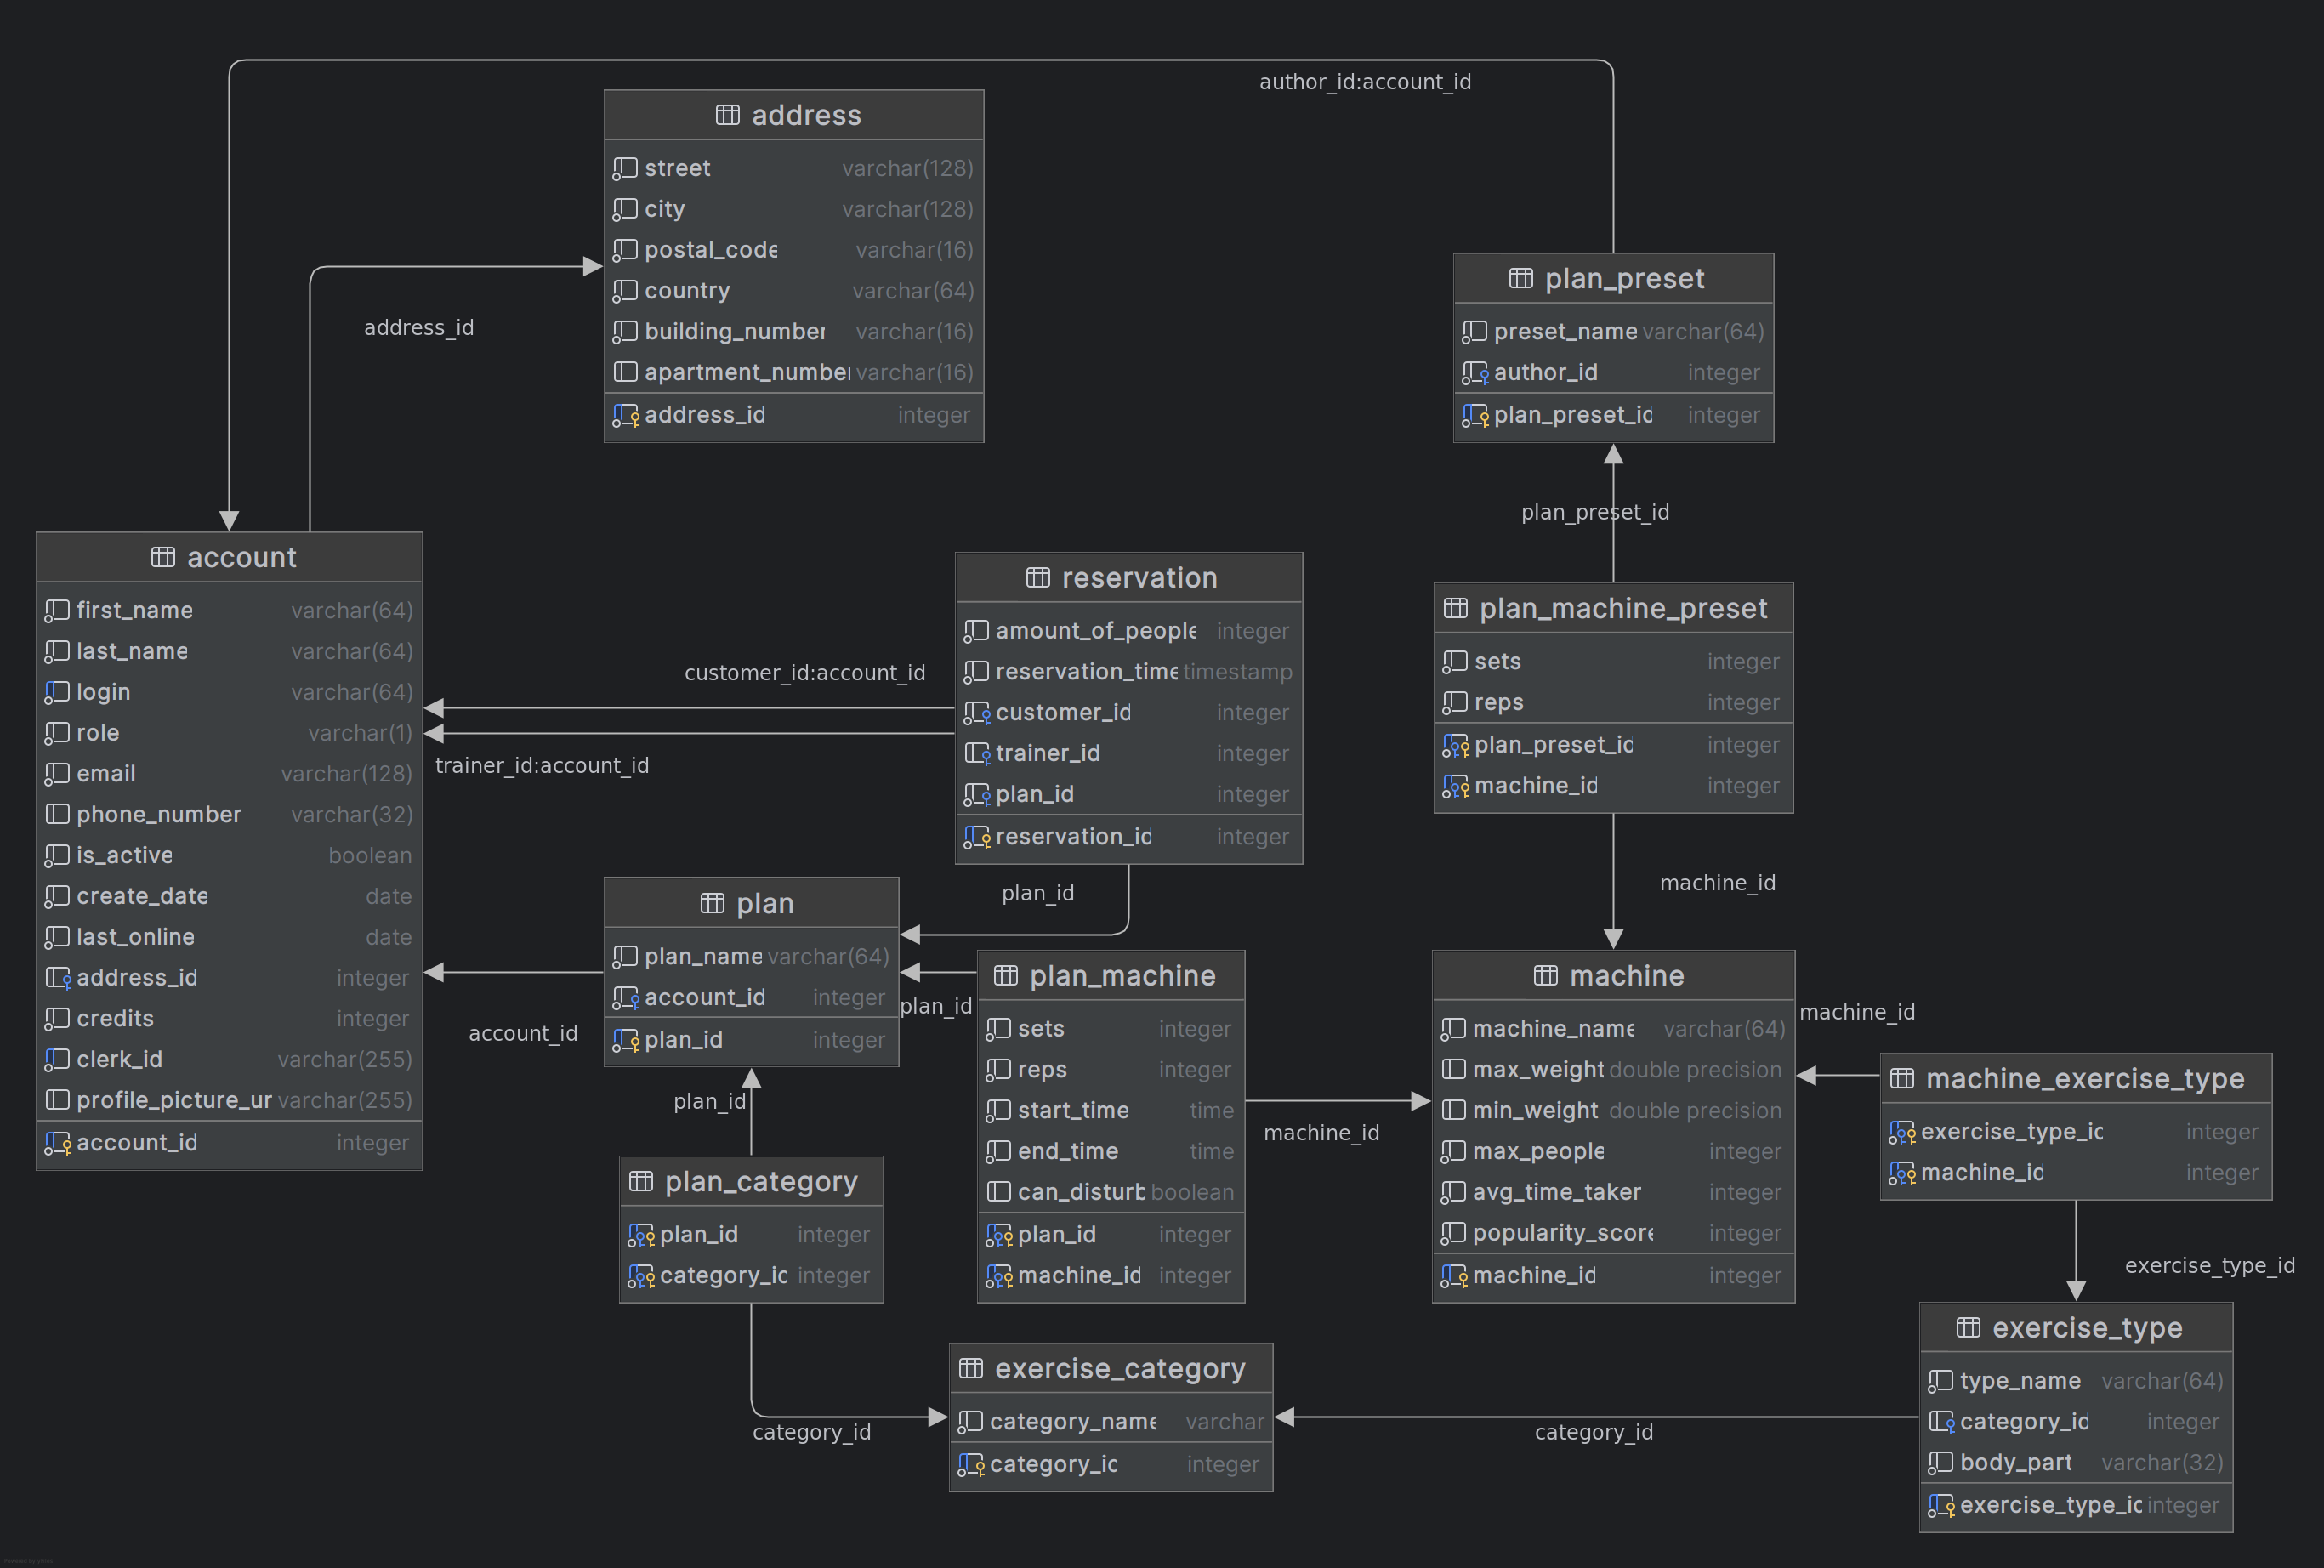
\includegraphics[width=1\textwidth]{Figures/ermodel.png}
	\caption{ Relační model}
	\label{fig:RelationalModel}
\end{figure}

\subsubsection{Popis dat}
Tato sekce se věnuje popisu nejdůležitějších tabulek, které můžeme vidět v ER-modelu. Jedná se o následující 4 tabulky: reservation (rezervace), machine (přístroj), plan (tréninkový plán), plan\_machine (slouží jako vztah mezi přístrojem a plánem, můžeme chápat jako reprezentaci časového okna). Ostatní tabulky slouží primárně k uchovávání doplňujících informací nebo ke správě relací mezi výše uvedenými tabulkami.

\begin{table}[h!]
	\caption{Popis databázové tabulky - reservation}
    \label{tab:dat-dictionary-reservation}
	\begin{tabular}{|p{3.5cm}|p{2cm}|p{1cm}|p{2.5cm}|p{.75cm}|p{3.75cm}|}
		\hline
        \textbf{Název atributu} & \textbf{Dat. Typ} & \textbf{Délka} & \textbf{Klíč} & \textbf{Null} & \textbf{Popis} \\
        \hline
        reservation\_id & INTEGER & - & Primární & Ne & Id rezervace \\
        \hline
        ammout\_of\_people & INTEGER & - & - & Ne & Počet lidí \\
        \hline
        reservation\_time & DATE & - & - & Ne & Čas příchodu \\
        \hline
        customer\_id & INTEGER & - & Cizí (account) & Ne & Id uživatele, na kterého je rezervace napsaná \\
        \hline
        trainer\_id & INTEGER & - & Cizí (account) & Ano & Id trenéra \\
        \hline
        plan\_id & INTEGER & - & Cizí (plan) & Ne & Id plánu \\
        \hline
	\end{tabular}
\end{table}

\begin{table}[h!]
	\caption{Popis databázové tabulky - machine}
    \label{tab:dat-dictionary-machine}
	\begin{tabular}{|p{3.5cm}|p{2cm}|p{1cm}|p{2.5cm}|p{.75cm}|p{3.75cm}|}
		\hline
        \textbf{Název atributu} & \textbf{Dat. Typ} & \textbf{Délka} & \textbf{Klíč} & \textbf{Null} & \textbf{Popis} \\
        \hline
            machine\_id & INTEGER   &  -    & Primární       & Ne & Id stroje \\
            \hline
            machine\_name     & VARCHAR   &  64   & -                 & Ne & Název stroje \\
            \hline
            max\_weight       & FLOAT   &  -   & -                 & Ne &  Maximální váha, kterou lze použít \\
            \hline
            min\_weight       & FLOAT   &  -    & -                 & Ne &  Minimální váha, kterou lze použít \\
            \hline
            max\_people       & INTEGER   &  -  & -                 & Ne & Maximální počet lidí na stroji \\
            \hline
            avg\_time\_taken    & INTEGER   &     & -                 & Ne & Průměrný trávený čas \\
            \hline
            popularity\_score & INTEGER      &  -    & -                 & Ne &  Počet rezervací \\
        \hline
	\end{tabular}
\end{table}

\begin{table}[h!]
	\caption{Popis databázové tabulky - plan}
    \label{tab:dat-dictionary-plan}
	\begin{tabular}{|p{3.5cm}|p{2cm}|p{1cm}|p{2.5cm}|p{.75cm}|p{3.75cm}|}
		\hline
        \textbf{Název atributu} & \textbf{Dat. Typ} & \textbf{Délka} & \textbf{Klíč} & \textbf{Null} & \textbf{Popis} \\
        \hline
            plan\_id & INTEGER   &  -    & Primární       & Ne & Id plánu \\
        \hline
            plan\_name     & VARCHAR   &  64   & -                 & Ne & Název plánu \\
        \hline
            account\_id     & INTEGER   &  -   & Cizí (account)                 & Ne & Id uživatele, který vytvořil plán \\
        \hline
	\end{tabular}
\end{table}

\begin{table}[h!]
	\caption{Popis databázové tabulky - plan\_machine}
    \label{tab:dat-dictionary-plan-machine}
	\begin{tabular}{|p{3.5cm}|p{2cm}|p{1cm}|p{2.5cm}|p{.75cm}|p{3.75cm}|}
		\hline
        \textbf{Název atributu} & \textbf{Dat. Typ} & \textbf{Délka} & \textbf{Klíč} & \textbf{Null} & \textbf{Popis} \\
        \hline
            plan\_id        & INTEGER   &  -    & Cizí (plan)       & Ne & Id plánu \\
        \hline
            machine\_id     & INTEGER   &  -    & Cizí (machine)       & Ne & Id stroje \\
        \hline
            sets                & INTEGER   &  -   & -                 & Ne & počet sérií\\
        \hline
            reps                & INTEGER   &  -    & -                 & Ne &  Počet opakování \\
        \hline
            start\_time     & TIME      &  -    & -                 & Ne & Čas začátku \\
        \hline
            end\_time       & TIME      &  -    & -                 & Ne & čas konce \\
        \hline
            can\_disturb          & BOOLEAN   &  =    & -                 & Ne & povolení kolizí \\
        \hline
	\end{tabular}
\end{table}

\subsubsection{Procedury a funkce}
Konkrétní procedury a funkce budou popsány v pozdější části této práce. Klíčovým aspektem návrhu je určení, které operace budou efektivnější realizovat na úrovni databáze a které na aplikační vrstvě. Toto rozhodnutí je zásadní, protože ovlivňuje nejen efektivitu a přehlednost řešení, ale také jeho dlouhodobou udržovatelnost.

Procedury a funkce jsou v kontextu navržené architektury využity pro extrakci komplexních datových struktur, nejsou však aplikovány pro jiné operace, jako například manipulace s daty, nebo~složitější transakce. Toto rozhodnutí vychází ze dvou východisek:

\begin{description}
    \item[Minimalizace funkcionality databázové vrstvy] 
    Databáze je využita především jako stabilní uložiště dat a optimalizovaný nástroj pro jejich vyhledávání. Transformace dat a obchodní logika je delegována na aplikační vrstvu.
    \item[Využití výhod aplikační vrstvy]
    Výhodou aplikační vrstvy oproti vrstvě datové je možnost využití obecných programovacích jazyků (např. JavaScript), které – na rozdíl od databázového jazyka PL/pgSQL – poskytují širší spektrum nástrojů pro manipulaci s daty, implementaci procedurální logiky a správu komplexních operací.  
\end{description}
Tento přístup přesouvá složitou obchodní logiku z databázové vrstvy do prostředí, které lépe odpovídá požadavkům na moderní softwarový vývoj. Zároveň toto rozhodnutí reflektuje princip separace zodpovědnosti (Separation of Concern - SoC), čímž ustanovuje jasné hranice mezi aplikační a datovou vrstvou, které následně vedou k více robustnímu a bezpečnému řešení. \cite{de2002importance}




\section{Backend}
Jedná se o HTTP rozhraní, které zajišťuje komunikaci mezi databází a uživatelským rozhraním. Rozhraní je napsáno v jazyce TypeScript, což přispívá k jazykové konzistenci napříč celým systémem a umožňuje využití moderních jazykových funkcí, včetně silné typové kontroly.

Pro práci s databází nebyly použity žádné existující knihovny pro implementaci ORM (Object-Relational Mapping). Místo toho jsem se rozhodl vytvořit vlastní implementaci ORM. Tento přístup poskytuje větší flexibilitu a kontrolu nad způsobem, jakým jsou data spravována a manipulována. Konkrétní detaily této implementace budou popsány v následujících sekcích.

\subsection{ORM}
Pro implementaci ORM jsem se rozhodl využít kombinaci reflexe a dekorátorů. Toto řešení mi umožnilo výrazně zjednodušit vývoj jednoduchých CRUD(tj. Create, Read, Update, Delete) operací pro jednotlivé koncové body. Výhodou tohoto přístupu je, že stačí definovat model, opatřit ho vhodnými dekorátory, a samotné mapování na SQL se následně provádí automaticky díky reflexi.

Důvodem rozhodnutí implementace vlastního ORM byla snaha o minimalizaci externích knihoven a jiných závislostí na straně backendu. Tento přístup poskytuje řadu výhod, například: lepší kontrolu nad kódem i jeho kvalitou, jednoznačnou zodpovědnost za případné chyby a mnohé další.

Konkrétní implementační detaily budou popsány v následující části.

\subsubsection{Dekorátory}
Dekorátory umožňují rozšířit funkcionalitu běžných tříd pomocí metadat nebo různých nadstaveb, které „dekorují“ danou třídu nebo její atributy\cite{TSDecorators}. V kontextu této práce byly tyto dekorátory implementovány přímo pro potřeby projektu, zejména pro přesné mapování objektových modelů na databázové tabulky a sloupce. Mezi naimplementovanými dekorátory vznikajícími přímo pro tuto architekturu lze rozlišit několik typů:
\begin{description}
    \item[Table] 
    Tento dekorátor slouží k přiřazení názvu tabulky dané třídě. Pomocí reflexe je název tabulky propojen s třídou, která ji reprezentuje, což usnadňuje práci při mapování modelů na SQL.
    \item[PrimaryKey]  
Dekorátor, který specifikuje primární klíč tabulky. Aplikace jej využívá pro identifikaci a práci s primárním klíčem záznamů v databázi.

\item[Column] 
Tento dekorátor přidává k atributům třídy odpovídající názvy sloupců v databázi. Zároveň přiřazuje daným atributům i specifické datové struktury v pozadí.

\item[ForeignKey] 
Dekorátor určený pro označení cizího klíče. Do dekorátoru se předává typ reprezentující odkazovanou tabulku, přičemž atribut, na který je dekorátor aplikován, musí být stejného typu. Navíc je nutné, aby odkazovaný typ dědil z obecné třídy \texttt{Model}.

\item[UnInsertable]
Označuje atributy, které mají být při vkládání dat do databáze ignorovány. Je využíváno pro zamezení vložení atributu, jejichž hodnota je nastavována skrze základní hodnoty v databázi. Například create\_date v tabulce account.

\item[DifferentlyNamedForeignKey]  
Používá se v případě, kdy atribut reprezentuje cizí klíč, ale jeho název se liší od názvu primárního klíče v odkazované tabulce. Tento dekorátor řeší situace, kdy databázová struktura neodpovídá standardnímu pojmenování. Například mějme cizí klíč \texttt{customer\_id}, který odkazuje na tabulku \texttt{account}, jenže PK má v dané tabulce název \texttt{account\_id}.

\item[UnUpdatable]  
Podobně jako \texttt{UnInsertable} tento dekorátor zajišťuje, že atributy označené tímto dekorátorem budou ignorovány při požadavku aktualizace dat.

\item[ManyToMany]
Dekorátor, který označuje atributy reprezentující vztah typu M:N (mnoho na mnoho) mezi dvěma tabulkami. Tento dekorátor umožňuje automatické zpracování spojovacích tabulek a souvisejících operací.
\end{description}


\subsection{Struktura}
Struktura projektu prošla několika výraznými změnami. S každou iterací systém nabýval na komplexitě a více strádal na přehlednosti, což vedlo k rozhodnutí provést kompletní přepsání backendu. Toto rozhodnutí vedlo k výraznému zlepšení přehlednosti a jednoduchosti systému. Podrobné poznámky k procesu refaktoringu a jednotlivým iteracím jsou uvedeny v následujících částech textu.

Aktuální backendová architektura je koncipována jako přehledně strukturované řešení s explicitním důrazem na logické uspořádání komponent. Její organizace je založená na seskupování zdrojů dle koncových bodů (např. rezervace, uživatelský účet, atd.), místo tradičního rozdělení podle funkcí (např. service, controller, atd.)
Kořenový adresář je uspořádán následujícím způsobem:
\dirtree{%
.1 db/.
.2 create\_script.sql.
.1 tests/.
.2 ....
.1 src/.
.2 database/.
.3 decorators/.
.4 database-decorators.ts.
.3 basic-query-database.ts.
.3 database-response.ts.
.3 database.ts.
.2 endpoints/.
.3 reservation/.
.4 reservation.controller.ts.
.4 reservation.database.ts.
.4 reservation.error-handler.ts.
.4 reservation.model.ts.
.4 reservation.routes.ts.
.4 reservation.service.ts.
.3 ....
.2 errors/.
.3 base.error.ts.
.3 error.handler.ts.
.2 request-utility/.
.3 common/.
.4 response-status.ts.
.3 custom-responses/.
.4 ok-response.ts.
.4 created-response.ts.
.4 ....
.2 router/.
.3 router.ts.
.2 utils/.
.3 ....
.2 app.ts.
.2 package.json.
.2 package-lock.json.
}
\subsection{Root složka}
\begin{description}
    \item[db] 
    Zde se ukládají SQL scripty pro vytvoření databáze, vkládání testovacích dat další podobné scripty.
    \item[tests]  
    Zde jsou uloženy testy napsány v pythonu pomocí knihovny pytest. Stručný popis testování můžete nalézt v kapitole \ref{testing&cicd}
    \item[src] 
    V této složce se nachází veškerá logika aplikace, která je podrobně popsána níže.
\end{description}

\subsection{Složka src}
Složka src centralizuje veškerou logiku Express.js HTTP serveru a je strukturována do následujících klíčových modulů:
\begin{description}
    \item[database] 
    Složka database obsahuje logiku specifickou pro ORM a obecné databázové operace. Jsou zde definovány nástroje, jako například výše zmíněné dekorátory pro mapování dat. Nachází se zde také typy reprezentující odpovědi z databáze, což zjednodušuje práci při manipulaci s daty.
    \item[endpoints]
    Každý koncový bod v projektu obsahuje následující soubory: controller, error-handler, model, routes a service. V některých případech může obsahovat i část database, která je zodpovědná za specifické databázové operace, jako jsou volání procedur nebo složité transakce.
    \item[errors] 
    Složka errors obsahuje základní error handler, ze kterého vycházejí ostatní handlery. Dále obsahuje definici typu CodedError, což je vlastní typ chyby obsahující kód chyby a odpovídající hlášku. Součástí je také ErrorCode, což je výčet chyb, které mohou nastat.
    \item[request-utility] 
    Složka request-utility obsahuje definice těl HTTP odpovědí, které se vrací z controllerů. Patří sem například:
    \texttt{CreatedResponse} pro úspěšné POST požadavky.
    \texttt{DeletedResponse} pro úspěšné DELETE požadavky.
    \item[router] 
    Router definuje všechny HTTP cesty, které API nabízí, a volá specifické routery pro jednotlivé endpointy.
    \item[utils] 
    Složka utils obsahuje pomocné funkce a typy, které usnadňují práci. Je zde například typ IDictionary (typová definice mapy pro libovolné datové typy), funkce safeAwait (funkce pro zjednodušení práce s try-catch. Umožňuje práci s chybami v podobném stylu jako v jazyce Go, což přispívá k přehlednosti kódu), definici loggeru (využívá PINO knihovnu) a pod.
    \item[app.ts] 
    Soubor app.ts slouží jako vstupní bod aplikace. Jeho hlavní funkcí je vytvoření instance frameworku express.js
\end{description} 

\subsection{Endpoints / Koncové body}
V další části popíšeme strukturu modulů a na příkladech ukážeme tok dat od rout přes aplikační logiku k databázi a zpět ke klientovi:

\subsubsection{Definice datové struktury - model}
Reprezentuje data vrácená v odpovědi. Model využívá dekorátory, které definují mapování mezi daty v modelu a databází. Jedná se o třídu, která dědí z obecného modelu.

\lstinputlisting[label=src:BEModel,caption={Příklad implementace endpoint modelu}]{SourceCodes/foo.model.ts}

Tento příklad demonstruje definiční datový model \texttt{Foo} s následující strukturou:
\begin{description}
    \item[FooId (typ number)] automaticky generovaný primární klíč tabulky
    \item[Bar (typ Bar)] cizí klíč definující 1:1 asociaci s tabulkou Bar.
\end{description} 

Model zároveň ilustruje aplikaci dekorátorů (např. \texttt{@PrimaryKey}, \texttt{@ForeignKey}, \texttt{@Column}, atd.), které rozšiřují funkcionalitu modelu o metadata nutná pro obecné požadavky na databázi. 

Následující příklad bude popisován dále v popisech dalších bodech.
\subsubsection{Definice koncových cest - routes}
Obsahuje definice HTTP cest, které se volají v globálním routeru. Tyto definice obvykle pouze směrují požadavky na příslušný controller.

\lstinputlisting[label=src:BERoutes,caption={Příklad implementace endpoint routů}]{SourceCodes/foo.routes.ts}

V tomto příkladu nejprve vytvoříme instanci \texttt{express.js} routeru. Následovně definujeme jednotlivé koncové body, které budou pro uživatele dostupné. Tyto definice pouze volají příslušný controller, kterému předává informace o requestu (dotazu) a o požadované response (odpovědi)

\subsubsection{Řízení aplikace a zpracování požadavků - controller} 
Zajišťuje logiku volání příslušných služeb (service) a sestavuje tělo HTTP odpovědi na základě výsledků těchto služeb.

\lstinputlisting[label=src:BEControllers,caption={Příklad implementace endpoint controllerů}]{SourceCodes/foo.controller.ts}

Kontroler \texttt{FooController} využívá \texttt{safeAwait} pro asynchronní error handling bez \texttt{try/catch}, inspirovaný jazykem \texttt{GO}. Metoda \texttt{FindById} nejprve načte entitu \texttt{Foo}, poté asociovaný \texttt{Bar}, a standardizuje odpovědi přes \texttt{OkResponse}/\texttt{FailedResponse}.

\subsubsection{Business logika a zpracování dat - service}
Úloha service je na základě vstupních dat vrátit data namapovaná na požadovaný typ. Tato data je možné získat z databáze, nebo z jiných služeb.

\lstinputlisting[label=src:BEServices,caption={Příklad implementace endpoint service}]{SourceCodes/foo.service.ts}

Příklad \texttt{FooService} ukazuje, jak metoda \texttt{GetFooById} využívá \texttt{BasicQueryDatabase} pro komunikaci s databází. Surová data z dotazu jsou transformována do instance třídy \texttt{Foo} pomocí explicitního mapování, které zajišťuje validaci a typovou bezpečnost.

\subsubsection{Práce s databází a specifické dotazy - database}
Pokud nejsou obecné operace pro práci v databázi pro potřebnou akci dostatečné, lze vytvořit instance databáze, která se od obecného řešení odvíjí, ale zároveň implementuje specifickou logiku vyžadovanou danými požadavky (dědí ze třídy \texttt{BasicQueryDatabase}).

\lstinputlisting[label=src:DBSelect,caption={Příklad implementace select funkce}]{SourceCodes/bd-select.ts}

\texttt{SelectSpecific} je jedna z funkcí třídy \texttt{BasicQueryDatabase}, která využívá metadata navázaná na objekt pomocí dekorátorů. Jak lze vidět, funkce se převážně jen stará o sestavení SQL dotazu, vrácení získaných dat a uzavření spojení s databází.

\subsubsection{error-handler}
Slouží jako mapper, který na základě vrácených chyb sestavuje odpovídající HTTP odpovědi. Pod pokličkou se jedná o hash mapu, která obsahuje typy chyb se status kódy. Je volán z controlleru.


% \subsection{Příklad}

\subsubsection{Model}
\lstinputlisting[label=src:BEModel,caption={Příklad implementace endpoint modelu}]{SourceCodes/foo.model.ts}

V ukázce je možné vidět praktické použití dekorátorů. Data, která potřebujeme inicializovat, jsou naplněna prostřednictvím konstruktoru. Konstruktor přijímá parametr typu IDictionary<any>, což je v podstatě HashMap, který umožňuje uchovávat hodnoty libovolného datového typu.


\subsubsection{Routes}

\subsubsection{Controller}


TODO

\subsubsection{Service}
\lstinputlisting[label=src:BEService,caption={TODO}]{SourceCodes/foo.service.ts}

TODO

\subsubsection{Database}
\lstinputlisting[label=src:BEDB,caption={TODO}]{SourceCodes/bd-select.ts}

TODO

\section{Frontend}
Frontend je uživatelské rozhraní aplikace, které interaguje s uživatelem a zobrazuje data z backendu. Je napsán ve Vue.js, což je moderní JavaScriptový framework pro vytváření uživatelských rozhraní. Frontend je koncipován mnohem jednodušeji. Hlavní funkčnost systému je na backendu, tudíž pro tvorbu uživatelského rozhraní je možné obejít předtím vytvořené pravidlo pro omezení ze strany externích knihoven. Systém Frontendovou část bere jako separátní aplikaci.

\subsubsection{Struktura}
Ve implementované Vue aplikaci je rozložena tímto způsobem:

\dirtree{%
.1 components/.
.2 Header/.
.3 Header.vue.
.3 MainNav.vue.
.3 ....
.2 ....
.1 views/.
.2 Admin/.
.2 pages/.
.3 Reservation/.
.4 Reservation.vue.
.4 ....
.3 ....
.2 ....
.2 Header/.
.3 Header.vue.
.3 MainNav.vue.
.3 ....
.2 ....
.1 router/.
.2 basic-routes/.
.2 reservation-router.ts.
.2 ....
.1 support/.
.2 services/.
.3 account.service.ts.
.3 ....
.2 types/.
.3 account.ts.
.3 ....	
.2 ....
.1 store/.
.2 accountStore.ts.
.2 ....
}


\begin{description}
    \item[Components] 

    \item[Views]  

    \item[support] 

    \item[router] 
    Aplikace vyuzívá vue router. To umožnuje implementaci veškerého routingu v jednom objektu. 

    \item[store]
    Pro ukládání globálního stavu, jako jsou například informace o přihlášeném uživateli jsoui využity tak zvané stores. Store je reaktivní proměnná, jež obsahuje nějakou hodnotu, kterou je potřeba přenést mezi několika komponentami.
\end{description}

Tato struktura je o něco více tradiční oproti backendu, ale jelikož se jedná o nižší komplexitu systému, tak není potřebné aplikovat přehlednější strukturu.

\subsubsection{Využité nástroje}
Jak již bylo zmíněno v sekci Využitých technologií, tak stylování bude využito Tailwind. Jelikož není vzhled UI pro tuto práci kritický, tak je využito ShadCn pro importování nastylovaných RADIX komponent přímo do projektu. Dále pro validaci vstupních parametrů formuláře bude využita knihovna zod.


